\chapter{Verwendete Technologien}\label{cha:used-technologies}

\section{Over The Air Update}\label{sec:ota}

\subsection*{Problemstellung}\label{sec:problem}
Der Workflow mit Mikrocontroller in Produktivsystemen ist aufwändig, da sie sich meist an ungünstigen Orten befinden. 
Bis jetzt musste man seine Datenquelle physisch mit dem Chip verbinden um neue Firmware auf den Mikrocontroller zu spielen. 
OTA ermöglicht es den Mikrocontroller mit neuer Firmware zu versorgen, dabei muss der ausgewählte Microcomputer lediglich mit einem Wlan-Router verbunden sein. 

\subsection*{Wie OTA funktioniert}
Am wichtigsten ist es, dass man die Partitionstabelle an das ausgewählte Programm anpasst. 
Die Standard-Partitionstabelle ist je nach Hersteller anders. Um OTA zu ermöglichen ist es notwendig im Partitionstabelle mindestens eine, ausreichend große, Partition zu vergeben. Dabei ist es wichtig, dass die OTA-Partition ausreichend Speicher für die gewünschte Firmware hat.

Damit der OTA-Vorgang funktionieren kann, muss zuerst ein lauffähiges Programm auf dem Mikrocontroller gestartet sein. Danach muss z.B. der ESP32 die neue Firmware über die bestehende Internet oder Intranet-Verbindung in die zuvor definierten Partition herunterladen. Anschließend muss nur noch der ESP32 mit der aktualisierten Partition neu gestartet werden. 

\subsection*{Implementation}
Die ausgewählte Struktur für die Diplomarbeit kann man im folgenden Bild sehr gut sehen.

\begin{figure}[H]
    \begin{center}
        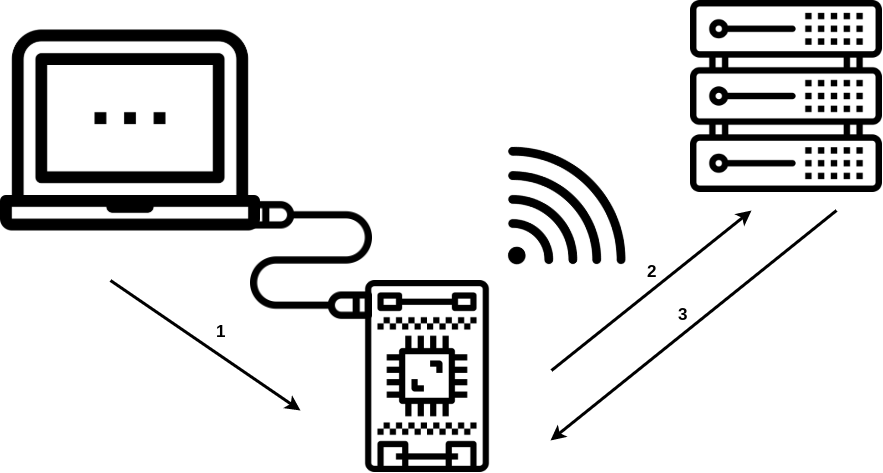
\includegraphics[scale=.5]{images/ota-explanation.png}
        \caption{OTA Erklärung (Quelle: eigene Darstellung)}
    \end{center}    
\end{figure}

\section{Mesh Netzwerk}\label{sec:mesh}

\section{Nodejs}\label{sec:nodejs}

\section{Platform IO}\label{sec:platformio}

\section{Docker}\label{sec:docker}

\section{Docker Compose}\label{sec:docker-compose}

\section{ESP IDF Utility lib}\label{sec:esp-idf-utility-lib}

\section{React}\label{sec:react}

\section{Yarn}\label{sec:yarn}

\section{Webpack}\label{sec:webpack}
